\documentclass[12pt, oneside]{article}
\usepackage[utf8]{inputenc}
\usepackage{polski}
\renewcommand*{\figurename}{Rys.}
\usepackage{graphicx}
\usepackage{float}
\usepackage{geometry}
\usepackage{subcaption}
\usepackage{indentfirst}
\usepackage{fancyvrb}
\setlength{\parindent}{4em}
\setlength{\parskip}{1em}
\geometry{
	left=25mm,
	right=25mm,%
	bindingoffset=10mm, 
	top=25mm, 
	bottom=25mm}
\title{
	Eksploracja Danych \\
	Światowy program szczepień przeciwko COVID-19
}
\author{
	Marek Grudkowski 156587
	\\
	Kamil Kaczmarkiewicz 171701
}

\begin{document}

\maketitle

\section{Krótki opis danych}

Zbiór danych dotyczy aktualnego postępu poszczególnych państw w szczepieniach przeciwko COVID-19. Zawiera on informacje pochodzące prawie ze wszystkich krajów na świecie podzielone na poszczególne dni. Większość atrybutów jest numeryczna i połączona ze sobą silną korelacją. Liczba przykładów z każdego kraju jest różna, co jest przedstawione na wykresie (Rysunek 1). 

\begin{figure}[h]
\centering
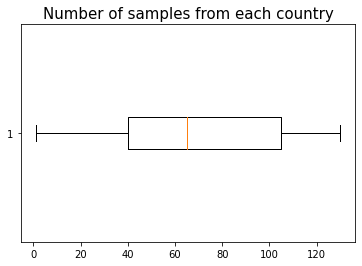
\includegraphics[width=0.6\textwidth]{../img/boxplot_of_samples.png} 
\caption{Liczba przykładów dostarczonych przez poszczególne państwa (pudełkowy)}
\label{Rys:samples}
\end{figure}


\section{Cele eksploracji danych}

Mając na uwadze, to czego dotyczy opisywany zbiór danych z łatwością można stwierdzić, że cel eksploracji miał związek z predykcją tego, jak program szczepień będzie przebiegał. Postawiliśmy w głównej mierze na, to aby:
\begin{itemize}
	\item wskazać państwa, które radzą sobie najlepiej w programie szczepień, by inne kraje mogły się na ich działaniach wzorować
	\item oszacować zapotrzebowanie w szczepionkach na nadchodzące miesiące, by uniknąć takich sytuacji jak brakujące czy marnujące się jej dawki (dokładność ok. 80\%)
	\item oszacować teoretyczną datę uzyskania przez dane państwo odporności zbiorowej
\end{itemize}

\subsection{Stopień pokrycia kryteriów sukcesu}

Pierwszy z celów został z łatwością osiągnięty. Wskazanie liderów w programie szczepień było bardzo prostym zadaniem i wymagało oprócz uprzedniego przygotowania danych, tylko wybrania tych państwa, w których krzywa ilości uodpornionych osób rosła najszybciej. Biorąc pod uwagę tylko ten fakt, na pierwszym miejscu pojawiały się państwa o bardzo małej liczbie ludności takiej jak San Marino, czy Gibraltar, gdzie szczepienia całego społeczeństwa można wykonać w ciągu kilku dni. W związku z tym braliśmy pod uwagę państwa, których populacja przekracza 8 milionów mieszkańców. Ostatecznie państwa, które są liderami  wprowadzaniu programu szczepień to: Zjednoczone Emiraty Arabskie, Izrael oraz Chile.

Drugi cel i trzeci cel wymagały zbudowania modelu, który mógłby przewidzieć na podstawie dotychczasowych danych jak program będzie przebiegał w przyszłości. Nasze prace oparliśmy na metodzie regresji wielomianowej i jak się potem okazało była ona nie tak dokładna jak powinna. 

Przykładowo dla Polski próbowaliśmy tą metodą przewidzieć zapotrzebowanie na szczepionki w pierwszej połowie maja. Różnica pomiędzy danymi uzyskanymi z predykcji, a tymi oryginalnymi zazwyczaj przekraczały 25\% rzeczywistej liczby podanych dawek. Widać też, że rozbieżność z każdym dniem rosła, co tym bardziej sprawia, że ten algorytm nie był zbyt dobrym rozwiązaniem.
 
\newpage

\begin{Verbatim}[tabsize=4]
date     pred     diff    [%]
01.05 - 238603 - 09199 - 03.86
02.05 - 227494 - 28815 - 12.67
03.05 - 207674 - 57476 - 27.68
04.05 - 223591 - 50745 - 22.70
05.05 - 219065 - 64809 - 29.58
06.05 - 223364 - 70410 - 31.52
07.05 - 247933 - 56112 - 22.63
08.05 - 256212 - 58483 - 22.83
09.05 - 261116 - 64619 - 24.75
10.05 - 280263 - 56910 - 20.31
11.05 - 281284 - 67735 - 24.08
12.05 - 299243 - 62039 - 20.73
13.05 - 301489 - 72483 - 24.04
14.05 - 299936 - 87163 - 29.06
15.05 - 300784 - 99889 - 33.29
\end{Verbatim}

\subsection{Ocena możliwości wykorzystania wyników w praktyce}

Wyznaczeni liderzy programu szczepień z pewnością mogą służyć za wzór. Dosyć głośno mówiło się o Izraelu (2 miejsce) czy USA (4 miejsce) i ich sprawnym programie prowadzenia szczepień. Dla nas bardzo dużym zaskoczeniem było to, że liderem światowym są Zjednoczone Emiraty Arabskie, a w czołówce są Chiny (5 miejsce) czy Chile (3 miejsce). 

Praktyki wykorzystywane przez kraje \textit{liderów} można z pewnością spróbować przyswoić w innych krajach. Zbadać jakie grupy osób były szczepione w jakiej kolejności, jak była prowadzona \textit{reklama} szczepień, czy były przewidziane ulgi dla osób zaszczepionych. Te wszystkie rzeczy z pewnością można wykorzystać w krajach, które pogram szczepień dopiero uruchamiają. 


\section{Wykonane prace}

Prace podczas eksploracji danych rozpoczęliśmy od eksploracyjnej analizy danych. Na jej podstawie poznaliśmy zależności pomiędzy atrybutami. Kluczowe było wówczas zauważenie, że pomiędzy atrybutami numerycznymi występują bardzo silne korelacje, jeśli bierzemy pod uwagę próbki z jednego państwa. Przy braniu pod uwagę wszystkich wierszy, problemem było to, że dla dużych krajów dzienna ilość podanych dawek była bardzo zbliżona do sumy podanych dawek w mniejszym kraju. Dlatego właśnie prace były wykonywane na próbkach z poszczególnych krajów. 

\newpage

Kluczowe też było zdanie sobie sprawy z ogromnych braków w danych. Podczas wykonywania analizy liczba brakujących wartości wyglądała tak jak na listingu poniżej:

\begin{verbatim}
Size of data is: (13307, 13)
Missing values in dataset: 
country                                   0
iso_code                                  0
date                                      0
total_vaccinations                     5255
people_vaccinated                      5931
people_fully_vaccinated                7926
daily_vaccinations_raw                 6529
daily_vaccinations                      220
total_vaccinations_per_hundred         5255
people_vaccinated_per_hundred          5931
people_fully_vaccinated_per_hundred    7926
daily_vaccinations_per_million          220
vaccines                                  0
\end{verbatim}

Podczas przygotowywania danych potrzeba było zatem dużo pracy, by doprowadzić zbiór do dobrego stanu. Większość wartości została wypełniona na podstawie interpolacji w kolumnie \textit{total vaccinations} gdyż byłą ona tak jakby atrybutem wyjściowym dla większości pozostałych. 

Po uzupełnieniu braków i standaryzowaniu zbioru rozpoczęliśmy pracę nad zbudowaniem modelu. Początkowo były to próby \textit{KNIME}, jednak po nieudanych próbach utworzenia poprawnego modelu postanowiliśmy wrócić do pisania skryptu w języku \textit{Python} oraz postawić na algorytm regresji wielomianowej. Po wykonaniu wielu eksperymentów w tym algorytmem z pewnością można stwierdzić, że nadrabia dokładność szybkością. W ciągu kilku minut potrafił dla każdego państwa sprawdzić wielomiany od 2 do 100 stopnia i określić, który zapewnia największą dokładność by następnie przeprowadzić predykcję osiągnięcia odporności populacyjnej. 

Niestety z tą dużą szybkością w parze szła też niedokładność. Rozbieżność przy testowaniu modelu dochodziła do 25\% i rosła z każdym kolejnym punktem oddalonym w przyszłość. Regresja wielomianowa nie jest zbyt dobrym narzędziem do predykcji ilości szczepień. Jest bardzo wrażliwa pod względem dobranego stopnia wielomianu i mimo niskiego błędu wpasowania, predykowane wartości znacznie odbiegają od tych, które w rzeczywistości się pojawią. Z pewnością bardziej skomplikowane algorytmy np. sieci neuronowe wydobyłyby z tego zbioru lepsze informacje. 

\begin{figure}[h!]
\centering
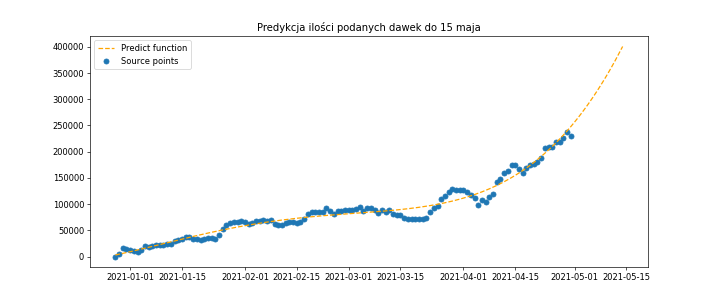
\includegraphics[height=0.25\textheight]{../img/demand1.png} 
\caption{Ambitna predykcja programu szczepień w Polsce}
\label{Rys:poland}
\end{figure}

\section{Znaczenie wyników dla przyszłej eksploracji}

Wykonane przez nas prace z pewnością mogą okazać się przydatne dla kogoś, kto posiadałby odpowiednią wiedzę i umiejętności, by skonstruować lepszy model do przewidywania zapotrzebowania na szczepionki. Dane zostały przez nas opracowane i wypełnione, a algorytm opisany i umieszczony w publicznym repozytorium, więc z tej strony może to oszczędzić przyszłym analitykom sporo pracy. 

Naszym głównym problemem okazało się dobranie nieodpowiedniego algorytmu do modelu. Według obliczeń jego dokładność na  zbiorze uczącym oscylowała w granicach od 95 do nawet 100 procent. Jednak, gdy do modelu został przekazany zbiór walidujący, wyszła na jaw jego niska skuteczność, która średnio wynosiła około 75\% i rosła z każdym kolejnym punktem oddalonym w przyszłość. 

Możliwe, że dobrym rozwiązaniem byłoby tutaj patrzenie nie na pojedyncze państwa i dane wyłącznie z tego jednego zbioru, lecz na cały świat z uwzględnieniem takich warunków jak produkt krajowy brutto, czy polityka państwa.

\end{document}
